\pagenumbering{arabic}
\setcounter{page}{1}
\renewcommand*{\thepage}{A\arabic{page}}
\appendix
\counterwithin{table}{section}
\counterwithin{figure}{section}

\section*{Appendix} % Add this line to create an unnumbered chapter title

\section{Estimation}

Throughout, we quantify prompt stability using Krippendorff's $\alpha$ (KA). For any set of annotations on the same items, Krippendorff's $\alpha$ is:
\[
\alpha \;=\; 1 - \frac{D_o}{D_e},
\]
where $D_o$ is observed disagreement and $D_e$ is expected disagreement under chance agreement given the marginal label distribution. For nominal (including binary) data, these quantities can be written as:
\[
D_o \;=\; \frac{1}{N} \sum_{c=1}^{n} \sum_{k=1}^{K} \sum_{l=1}^{K} o_{ck}\, o_{cl}\, d_{kl},
\qquad
D_e \;=\; \frac{1}{N(N-1)} \sum_{k=1}^{K} \sum_{l=1}^{K} e_{k}\, e_{l}\, d_{kl},
\]
where $o_{ck}$ is the number of raters assigning category $k$ to item $c$, $e_k$ is the total number of assignments of category $k$ across all items, $d_{kl}$ is the distance between categories $k$ and $l$ (for nominal data, $d_{kl}= \mathbb{I}[k\neq l]$), $K$ is the number of categories, $n$ is the number of items, and $N$ is the total number of rater--item assignments.\footnote{For interval outcomes we use an interval distance (typically squared differences). The implementation uses \texttt{simpledorff}'s nominal or interval metric as appropriate.}

\subsection{Intra-prompt stability (intra-PSS)}

Let $D=\{x_i\}_{i=1}^{n}$ denote the (subsampled) dataset items to be annotated. Fix a single prompt $p$ (optionally $p = \texttt{original\_text} + \texttt{prompt\_postfix}$). The scratch algorithm and the Python implementation treat \emph{repeated runs of the same prompt} as the ``raters.''

Let
\[
C_{i,r}
\]
denote the label produced for item $i$ on run $r$, for $i=1,\ldots,n$ and $r=1,\ldots,R$ (where in the paper we typically set $R=30$; in the package examples this is user-specified via \texttt{iterations}).

After collecting annotations for runs $1,\ldots,r$, the cumulative intra-prompt stability estimate is computed as Krippendorff's $\alpha$ across runs (i.e., across ``raters'') on the same items:
\[
\alpha^{\mathrm{cum}}_r
\;=\;
KA\!\left(
\left\{\, C_{i,1},\, C_{i,2},\, \ldots,\, C_{i,r} \,\right\}_{i=1}^{n}
\right),
\qquad r \ge 2.
\]
In words: for each item $i$, we have $r$ labels from $r$ repeated runs; we compute KA over this item-by-run annotation matrix. This produces the cumulative intra-PSS sequence $\{\alpha^{\mathrm{cum}}_r\}_{r=2}^{R}$.

We also report a complementary adjacent-run diagnostic:
\[
\alpha^{\mathrm{adj}}_r
\;=\;
KA\!\left(
\left\{\, C_{i,r-1},\, C_{i,r} \,\right\}_{i=1}^{n}
\right),
\qquad r \ge 2.
\]
This statistic uses only the labels from runs $r-1$ and $r$, so it captures local run-to-run volatility rather than cumulative convergence. In the revised workflow, the intra-PSS output is therefore the pair of sequences $\{\alpha^{\mathrm{cum}}_r\}_{r=2}^{R}$ and $\{\alpha^{\mathrm{adj}}_r\}_{r=2}^{R}$.

\paragraph{Bootstrapped uncertainty (as implemented).}
To form confidence intervals, the Python code bootstraps by resampling the \emph{annotation records} with replacement from the long-format table of annotations and recomputing KA on each resample. Concretely, let
\[
\mathcal{A}_{\le r} \;=\; \{(i, s, C_{i,s}) : i=1,\ldots,n,\; s=1,\ldots,r\}
\]
denote the set of annotation records up to run $r$ (represented in the code as the subset of rows with \texttt{iteration} $\le r$). For bootstrap draw $b=1,\ldots,B$, the code samples
\[
\mathcal{A}^{(b)}_{\le r} \sim \text{SampleWithReplacement}\bigl(\mathcal{A}_{\le r},\ |\mathcal{A}_{\le r}|\bigr),
\]
computes
\[
\alpha^{(b)}_r \;=\; KA\!\left(\mathcal{A}^{(b)}_{\le r}\right),
\]
and then reports the bootstrap mean and percentile confidence interval:
\[
\widehat{\alpha}_r \;=\; \frac{1}{B}\sum_{b=1}^{B}\alpha^{(b)}_r,
\qquad
\text{CI}_{r,\,0.95} \;=\; \left[\, Q_{0.025}(\{\alpha^{(b)}_r\}),\; Q_{0.975}(\{\alpha^{(b)}_r\}) \,\right].
\]
This matches the package routine \texttt{bootstrap\_krippendorff} used inside \texttt{intra\_pss}. For the adjacent-run statistic, the same bootstrap is applied to the restricted long-format record set
\[
\mathcal{A}^{\mathrm{adj}}_{r} \;=\; \{(i, s, C_{i,s}) : i=1,\ldots,n,\; s\in\{r-1,r\}\},
\]
yielding bootstrap draws
\[
\alpha^{(b),\mathrm{adj}}_r \;=\; KA\!\left(\mathcal{A}^{(b),\mathrm{adj}}_{r}\right).
\]
When we visualize adjacent-run confidence intervals, the reported upper endpoint is bounded above at $1$, the logical maximum of Krippendorff's $\alpha$.

\subsection{Inter-prompt stability (inter-PSS)}

For inter-prompt stability, the scratch algorithm and the Python implementation treat \emph{prompt variants} (generated at a fixed paraphraser temperature) as the ``raters.''

Let $\mathcal{T}$ be the set of paraphraser temperatures. For each $t\in\mathcal{T}$, the code generates $V$ prompt variants
\[
p_{t,1},\, p_{t,2},\, \ldots,\, p_{t,V},
\]
where, in the current implementation, $V = 1 + \texttt{nr\_variations}$ because the list includes the original prompt as one variant plus $nr\_variations$ paraphrases.

For each temperature $t$ and variant $v$, the annotation function is applied to each item $x_i$. Let
\[
C_{i,t,v}
\]
denote the label for item $i$ produced under variant $v$ at paraphraser temperature $t$.

Then inter-prompt stability at temperature $t$ is computed as Krippendorff's $\alpha$ across variants (i.e., across ``raters'') on the same items:
\[
\alpha_t
\;=\;
KA\!\left(
\left\{\, C_{i,t,1},\, C_{i,t,2},\, \ldots,\, C_{i,t,V} \,\right\}_{i=1}^{n}
\right).
\]
The inter-PSS output is the curve $\{(t,\alpha_t)\}_{t\in\mathcal{T}}$.

\paragraph{Multiple annotation repetitions (what the code does).}
The \texttt{inter\_pss} function has an argument \texttt{iterations}. In the common use case (and in our paper figures), we set \texttt{iterations}=1, so each $(i,t,v)$ is annotated once and the notation above is exact.

If \texttt{iterations} $>1$, the current Python implementation appends additional annotation records but does \emph{not} store an explicit repetition index in the output table. KA is then computed on the pooled long-format records with \texttt{annotator\_col} set to \texttt{prompt\_id}. In other words, the estimator remains ``KA across prompt variants within temperature,'' but repeated records for the same $(i,t,v)$ are included as additional rows rather than being aggregated into a single $\widetilde{C}_{i,t,v}$ via a defined rule. (If you want a strict ``one rating per rater per item'' design under repeats, you would need to add an explicit repetition index and an aggregation rule; the present section documents the implementation as-is.)

\paragraph{Bootstrapped uncertainty (as implemented).}
Within each temperature $t$, the code bootstraps by resampling the long-format annotation records for that temperature with replacement, recomputing KA each time. Let
\[
\mathcal{A}_t \;=\; \{(i, v, C_{i,t,v}) : i=1,\ldots,n,\; v=1,\ldots,V\}
\]
denote the set of annotation records at temperature $t$ (represented in the code as \texttt{annotated\_data} for that temperature). For $b=1,\ldots,B$:
\[
\mathcal{A}^{(b)}_{t} \sim \text{SampleWithReplacement}\bigl(\mathcal{A}_t,\ |\mathcal{A}_t|\bigr),
\qquad
\alpha^{(b)}_t = KA\!\left(\mathcal{A}^{(b)}_{t}\right),
\]
and the routine reports the bootstrap mean and percentile confidence interval:
\[
\widehat{\alpha}_t \;=\; \frac{1}{B}\sum_{b=1}^{B}\alpha^{(b)}_t,
\qquad
\text{CI}_{t,\,0.95} \;=\; \left[\, Q_{0.025}(\{\alpha^{(b)}_t\}),\; Q_{0.975}(\{\alpha^{(b)}_t\}) \,\right].
\]
This matches \texttt{bootstrap\_krippendorff} as called inside \texttt{inter\_pss} (with \texttt{annotator\_col} set to \texttt{prompt\_id} and \texttt{experiment\_col} set to \texttt{id}).


\section{Bootstrapping}

We quantify uncertainty in Krippendorff's $\alpha$ using a nonparametric bootstrap. In both the intra- and inter-prompt routines, we work with a long-format annotation table where each row is an annotation record (item id, rater id, and label). For each bootstrap replicate, we resample annotation records with replacement, recompute $\alpha$ on the resampled table, and form percentile confidence intervals from the resulting empirical distribution.

\subsection{Intra-prompt stability}

Let $\mathcal{A}_{\le r}$ denote the set of annotation records obtained after $r$ runs of the fixed prompt (so raters correspond to runs). For each bootstrap replicate $b=1,\ldots,B$, we draw a resample
\[
\mathcal{A}^{(b)}_{\le r} \sim \text{SampleWithReplacement}\!\left(\mathcal{A}_{\le r},\, |\mathcal{A}_{\le r}|\right),
\]
compute
\[
\alpha^{(b)}_{r} = KA\!\left(\mathcal{A}^{(b)}_{\le r}\right),
\]
and report the bootstrap mean and a $95\%$ percentile interval:
\[
\widehat{\alpha}_{r}=\frac{1}{B}\sum_{b=1}^{B}\alpha^{(b)}_{r},
\qquad
\text{CI}_{r,0.95}=\left[Q_{0.025}(\{\alpha^{(b)}_{r}\}),\, Q_{0.975}(\{\alpha^{(b)}_{r}\})\right].
\]
For the adjacent-run diagnostic, we repeat the same procedure on
\[
\mathcal{A}^{\mathrm{adj}}_{r}=\{(i,s,C_{i,s}): i=1,\ldots,n,\; s\in\{r-1,r\}\},
\]
which yields
\[
\widehat{\alpha}^{\mathrm{adj}}_{r}=\frac{1}{B}\sum_{b=1}^{B}\alpha^{(b),\mathrm{adj}}_{r},
\qquad
\text{CI}^{\mathrm{adj}}_{r,0.95}=\left[Q_{0.025}(\{\alpha^{(b),\mathrm{adj}}_{r}\}),\, \min\!\left(Q_{0.975}(\{\alpha^{(b),\mathrm{adj}}_{r}\}),\,1\right)\right].
\]

\subsection{Inter-prompt stability}

Fix a paraphraser temperature $t$ and let $\mathcal{A}_{t}$ denote the set of annotation records produced by applying each of the $V$ prompt variants at temperature $t$ to the same $n$ items (so raters correspond to prompt variants). For each bootstrap replicate $b=1,\ldots,B$, we draw
\[
\mathcal{A}^{(b)}_{t} \sim \text{SampleWithReplacement}\!\left(\mathcal{A}_{t},\, |\mathcal{A}_{t}|\right),
\]
compute
\[
\alpha^{(b)}_{t} = KA\!\left(\mathcal{A}^{(b)}_{t}\right),
\]
and report
\[
\widehat{\alpha}_{t}=\frac{1}{B}\sum_{b=1}^{B}\alpha^{(b)}_{t},
\qquad
\text{CI}_{t,0.95}=\left[Q_{0.025}(\{\alpha^{(b)}_{t}\}),\, Q_{0.975}(\{\alpha^{(b)}_{t}\})\right].
\]


\begin{algorithm}[t]
\caption{Prompt Stability Scoring (PSS): where Krippendorff's $\alpha$ is computed (with bootstrap matching Python implementation)}
\label{alg:pss_ka_where_bootstrap_python}
\begin{algorithmic}[1]
\Require Items $\{x_i\}_{i=1}^n$, annotation function $f(\cdot,\cdot)$, distance metric $d(\cdot,\cdot)$ for KA
\Require (Intra) prompt $p$ and number of runs $J$
\Require (Inter) base prompt $p_0$, temperatures $\mathcal{T}$, variants per temperature $V$
\Require Bootstrap samples $B$ (optional)
\vspace{2mm}

\Statex \textbf{Intra-prompt stability (intra-PSS)}
\State Initialize long-format annotation table $\mathcal{A} \gets \emptyset$
\Comment{Each row is a record $(i,\texttt{run}=j, y)$}
\For{$j = 1$ \textbf{to} $J$}
    \For{$i = 1$ \textbf{to} $n$}
        \State $y \gets f(x_i, p)$
        \State Append record $(i, j, y)$ to $\mathcal{A}$
    \EndFor
    \If{$j \ge 2$}
        \State \textbf{Compute Krippendorff's $\alpha$ across runs (raters)}:
        \State \hspace{5mm} $\alpha_j \gets KA\!\left(\mathcal{A}_{\le j};\, d\right)$
        \Comment{$\mathcal{A}_{\le j}$ are records with $\texttt{run}\le j$}
        \If{$B > 0$}
            \For{$b = 1$ \textbf{to} $B$}
                \State Sample annotation records with replacement:
                \State \hspace{5mm} $\mathcal{A}^{(b)}_{\le j} \sim \text{SampleWithReplacement}\!\left(\mathcal{A}_{\le j},\,|\mathcal{A}_{\le j}|\right)$
                \State $\alpha^{(b)}_j \gets KA\!\left(\mathcal{A}^{(b)}_{\le j};\, d\right)$
            \EndFor
            \State Form percentile CI for $\alpha_j$ from $\{\alpha^{(b)}_j\}_{b=1}^B$
            \State (Optionally) report bootstrap mean $\widehat{\alpha}_j = \frac{1}{B}\sum_{b=1}^B \alpha^{(b)}_j$
        \EndIf
    \EndIf
\EndFor
\Statex \Comment{Output: sequence $\{\alpha_j\}_{j=2}^J$ (and CIs if bootstrapped)}

\vspace{3mm}
\Statex \textbf{Inter-prompt stability (inter-PSS)}
\For{\textbf{each} paraphraser temperature $t \in \mathcal{T}$}
    \State Generate prompt variants $\{p_{t,v}\}_{v=1}^{V}$ (optionally include $p_0$ as one variant)
    \State Initialize long-format annotation table $\mathcal{A}_t \gets \emptyset$
    \Comment{Each row is a record $(i,\texttt{variant}=v, y)$ at temperature $t$}
    \For{$v = 1$ \textbf{to} $V$}
        \For{$i = 1$ \textbf{to} $n$}
            \State $y \gets f(x_i, p_{t,v})$
            \State Append record $(i, v, y)$ to $\mathcal{A}_t$
        \EndFor
    \EndFor
    \State \textbf{Compute Krippendorff's $\alpha$ across prompt variants (raters), within temperature $t$}:
    \State \hspace{5mm} $\alpha_t \gets KA\!\left(\mathcal{A}_t;\, d\right)$
    \If{$B > 0$}
        \For{$b = 1$ \textbf{to} $B$}
            \State Sample annotation records with replacement:
            \State \hspace{5mm} $\mathcal{A}^{(b)}_{t} \sim \text{SampleWithReplacement}\!\left(\mathcal{A}_t,\,|\mathcal{A}_t|\right)$
            \State $\alpha^{(b)}_t \gets KA\!\left(\mathcal{A}^{(b)}_{t};\, d\right)$
        \EndFor
        \State Form percentile CI for $\alpha_t$ from $\{\alpha^{(b)}_t\}_{b=1}^B$
        \State (Optionally) report bootstrap mean $\widehat{\alpha}_t = \frac{1}{B}\sum_{b=1}^B \alpha^{(b)}_t$
    \EndIf
\EndFor
\Statex \Comment{Output: curve $\{(t,\alpha_t)\}_{t\in\mathcal{T}}$ (and CIs if bootstrapped)}
\end{algorithmic}
\end{algorithm}



\section{Additional figures}

\begin{landscape}
\begin{figure}[ht]
    \centering
    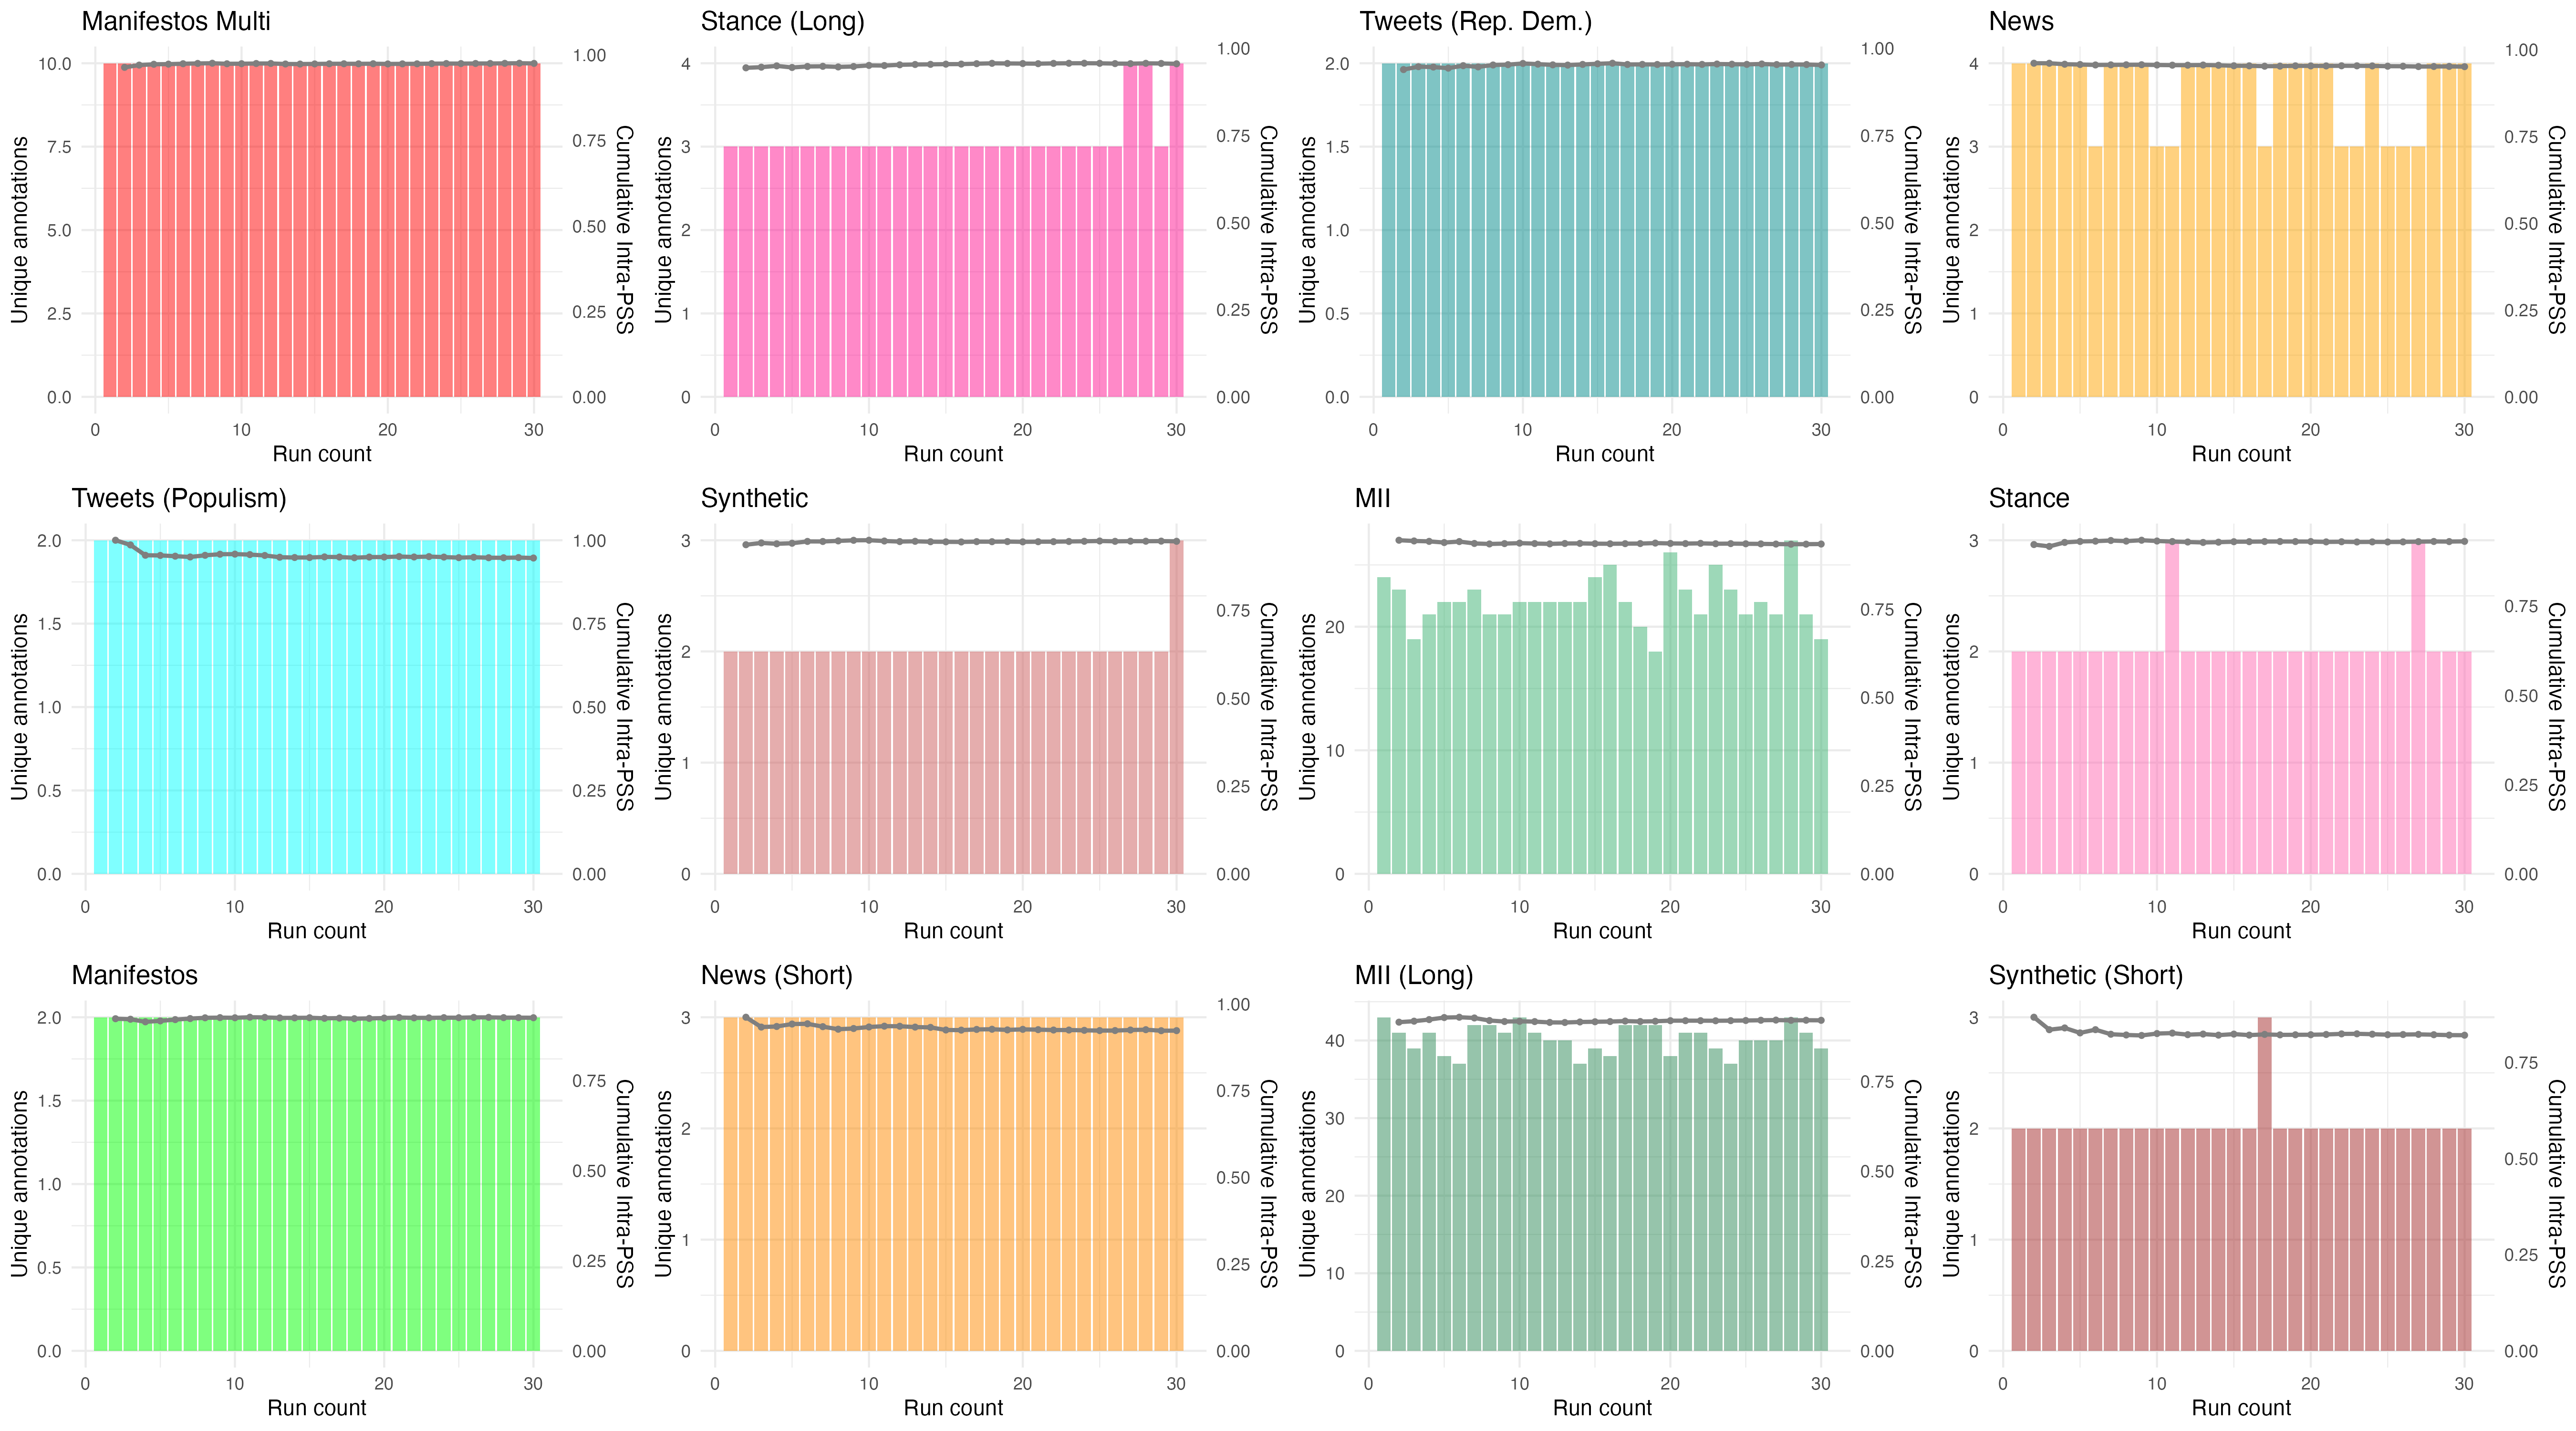
\includegraphics[width=1.2\textwidth]{plots/combined_postpro_within_diagnostics.png}
    \caption{Unique annotations by dataset and iteration.}
    \label{fig:combined_postpro_within_diagnostics}
\end{figure}

\begin{figure}[ht]
    \centering
    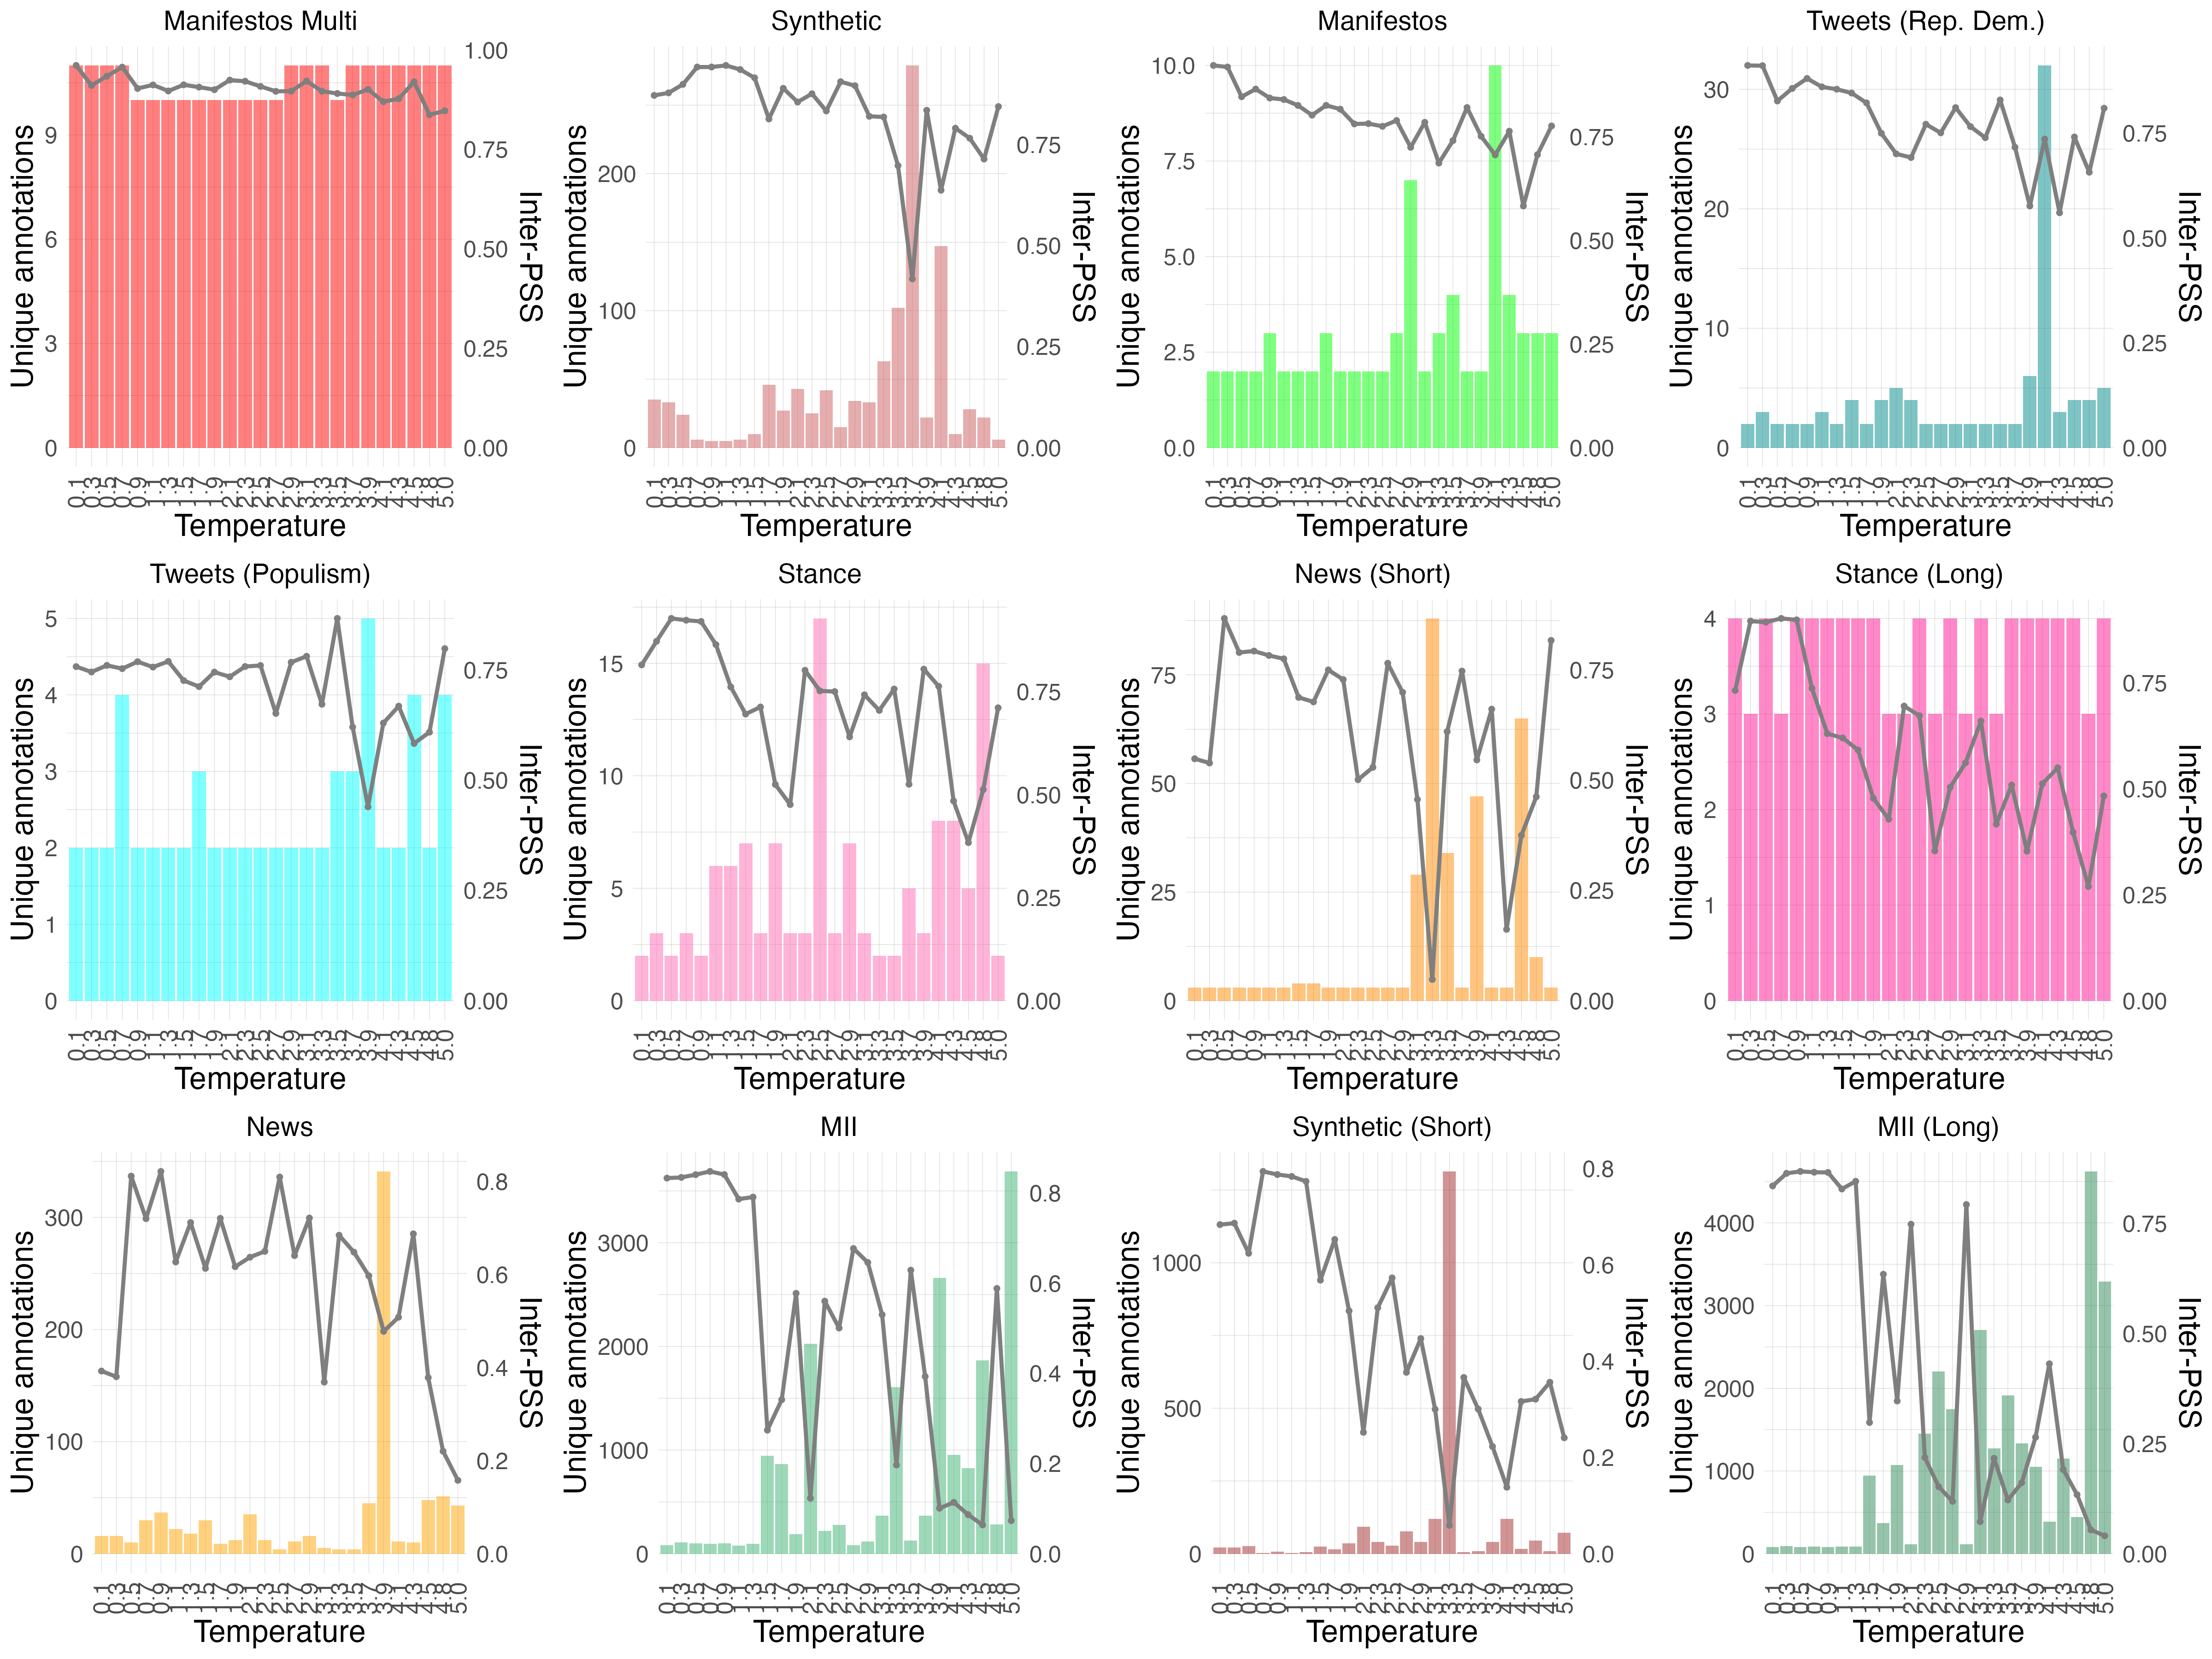
\includegraphics[width=1.2\textwidth]{plots/combined_postpro_between_diagnostics.png}
    \caption{Unique annotations by dataset and temperature.}
    \label{fig:combined_postpro_between_diagnostics}
\end{figure}

\end{landscape}

\section{LM Costs}

\begin{landscape}
  \begin{table}[!h]
    \centering
    \resizebox{\ifdim\width>\linewidth\linewidth\else\width\fi}{!}{%
      \begin{tabular}{lrrrr}
        \toprule
        Dataset           & Total Rows & Input tokens total & Output tokens total & Avg.\ tokens/call \\
        \midrule
        Manifestos        & 276{,}347    & 25{,}968{,}922           & 276{,}347              & 94               \\
        Manifestos Multi  & 276{,}201    & 25{,}954{,}819           & 276{,}201              & 94               \\
        MII               & 251{,}378    & 458{,}994             & 251{,}378              & 2                \\
        MII (Long)        & 233{,}670    & 462{,}566             & 233{,}670              & 2                \\
        News              & 409{,}734    & 198{,}099{,}296          & 409{,}734              & 483              \\
        News (Short)      & 84{,}451     & 10{,}257{,}657           & 84{,}451               & 121              \\
        Stance            & 412{,}362    & 6{,}881{,}473            & 412{,}362              & 17               \\
        Stance (Long)     & 264{,}775    & 4{,}459{,}825            & 264{,}775              & 17               \\
        Synthetic         & 395{,}563    & 16{,}240{,}554           & 395{,}563              & 41               \\
        Synthetic (Short) & 374{,}733    & 11{,}604{,}411           & 374{,}733              & 31               \\
        Tweets (Populism) & 82{,}405     & 3{,}001{,}132            & 82{,}405               & 36               \\
        Tweets (Rep. Dem.)& 82{,}403     & 3{,}001{,}306            & 82{,}403               & 36               \\
        Total             & 3{,}144{,}022   & 306{,}390{,}955          & 3{,}144{,}022             & ---              \\
        \bottomrule
      \end{tabular}%
    }
    \caption{Total size and tokens by dataset}
    \label{table:dataset_stats}
  \end{table}
  
  \vspace{2em}
  
  \begin{table}[!h]
    \centering
    \resizebox{\ifdim\width>\linewidth\linewidth\else\width\fi}{!}{%
      \begin{tabular}{lrrrrrrrrr}
        \toprule
        Dataset           & Input cost & Output cost & Total cost & 2\%  & 5\%   & 10\%  & 25\%  & 50\%  & 75\% \\
        \midrule
        Manifestos        & \$12.98      & \$0.41        & \$13.40      & 5{,}527 & 13{,}817 & 27{,}635 & 69{,}087 & 138{,}174 & 207{,}260 \\
        Manifestos Multi  & \$12.98      & \$0.41        & \$13.39      & 5{,}524 & 13{,}810 & 27{,}620 & 69{,}050 & 138{,}100 & 207{,}151 \\
        MII               & \$0.23       & \$0.38        & \$0.61       & 5{,}028 & 12{,}569 & 25{,}138 & 62844 & 125{,}689 & 188{,}534 \\
        MII (Long)        & \$0.23       & \$0.35        & \$0.58       & 4{,}673 & 11{,}684 & 23{,}367 & 58418 & 116{,}835 & 175{,}252 \\
        News              & \$99.05      & \$0.61        & \$99.66      & 8{,}195 & 20{,}487 & 40{,}973 & 102{,}434 & 204{,}867 & 307{,}300 \\
        News (Short)      & \$5.13       & \$0.13        & \$5.26       & 1{,}689 & 4{,}223  & 8{,}445  & 21{,}113  & 42{,}226  & 63{,}338  \\
        Stance            & \$3.44       & \$0.62        & \$4.06       & 8{,}247 & 20{,}618 & 41{,}236 & 103{,}090 & 206{,}181 & 309{,}272 \\
        Stance (Long)     & \$2.23       & \$0.40        & \$2.63       & 5{,}296 & 13{,}239 & 26{,}478 & 66{,}194  & 132{,}388 & 198{,}581 \\
        Synthetic         & \$8.12       & \$0.59        & \$8.71       & 7{,}911 & 19{,}778 & 39{,}556 & 98{,}891  & 197{,}782 & 296{,}672 \\
        Synthetic (Short) & \$5.80       & \$0.56        & \$6.36       & 7{,}495 & 18{,}737 & 37{,}473 & 93{,}683  & 187{,}366 & 281{,}050 \\
        Tweets (Populism) & \$1.50       & \$0.12        & \$1.62       & 1{,}648 & 4{,}120  & 8{,}240  & 20{,}601  & 41{,}202  & 61{,}804  \\
        Tweets (Rep. Dem.)& \$1.50       & \$0.12        & \$1.62       & 1{,}648 & 4{,}120  & 8{,}240  & 20{,}601  & 41{,}202  & 61{,}802  \\
        Total             & \$153.20     & \$4.72        & \$157.91     & \$3.16 & \$7.90  & \$15.79 & \$39.48  & \$78.96  & \$118.43 \\
        \bottomrule
      \end{tabular}%
    }
    \caption{Cost estimates for each dataset by percentile. Note these costs are current as of August, 2025 but provide a general rough estimate.}
    \label{table:costs_percentiles}
  \end{table}
\end{landscape}

\begin{table}[!h]
\centering
\caption{Estimated Total API Cost for Various Models}
\centering
\resizebox{\ifdim\width>\linewidth\linewidth\else\width\fi}{!}{
\begin{tabular}[t]{lrrlll}
\toprule
Model & input\_price & output\_price & cost\_input & cost\_output & total\_cost\\
\midrule
gpt-4o-mini & 0.15 & 0.60 & 45.96 & 1.89 & 47.85\\
gpt-4o & 2.50 & 10.00 & 765.98 & 31.44 & 797.42\\
o1-mini & 1.10 & 4.40 & 337.03 & 13.83 & 350.86\\
o1 & 15.00 & 60.00 & 4595.86 & 188.64 & 4784.51\\
o3-mini & 1.10 & 4.40 & 337.03 & 13.83 & 350.86\\
\addlinespace
claude-3.5-haiku & 0.80 & 4.00 & 245.11 & 12.58 & 257.69\\
claude-3.5-sonnet & 3.00 & 15.00 & 919.17 & 47.16 & 966.33\\
deepseek-v3 & 0.14 & 0.28 & 42.89 & 0.88 & 43.78\\
deepseek-r1 & 0.55 & 2.19 & 168.52 & 6.89 & 175.4\\
gemini-1.5-flash & 0.15 & 0.60 & 45.96 & 1.89 & 47.85\\
\addlinespace
gemini-1.5-pro & 1.25 & 5.00 & 382.99 & 15.72 & 398.71\\
mistral-small & 0.20 & 0.60 & 61.28 & 1.89 & 63.16\\
mistral-large & 2.00 & 6.00 & 612.78 & 18.86 & 631.65\\
\bottomrule
\end{tabular}}
\label{table:altlmcosts}
\end{table}

\section{Additional analyses}

\subsection{Filtered diagnostic comparisons}

In the main text, we treat filtering as a practical diagnostic rather than as a separate theoretical source of instability. Here we report the full filtered comparisons. We apply two procedures. First, we remove annotations that do not match the required integer format specified in the \texttt{prompt\_postfix}. Second, we construct a filtered and balanced dataset in which each iteration or temperature retains only as many rows as the smallest valid subset after filtering. This allows us to compare the original results to versions in which malformed outputs have been removed, with and without balancing the sample across iterations or temperatures.

The main takeaway is that these comparisons are diagnostic rather than substantive in themselves. For MII, filtering substantially improves both intra- and inter-PSS, suggesting that much of the apparent instability is driven by output-format errors. For Synthetic (Short), by contrast, filtering has little effect, indicating that the underlying task remains unstable even after malformed outputs are removed.

\begin{figure}[ht]
    \centering
    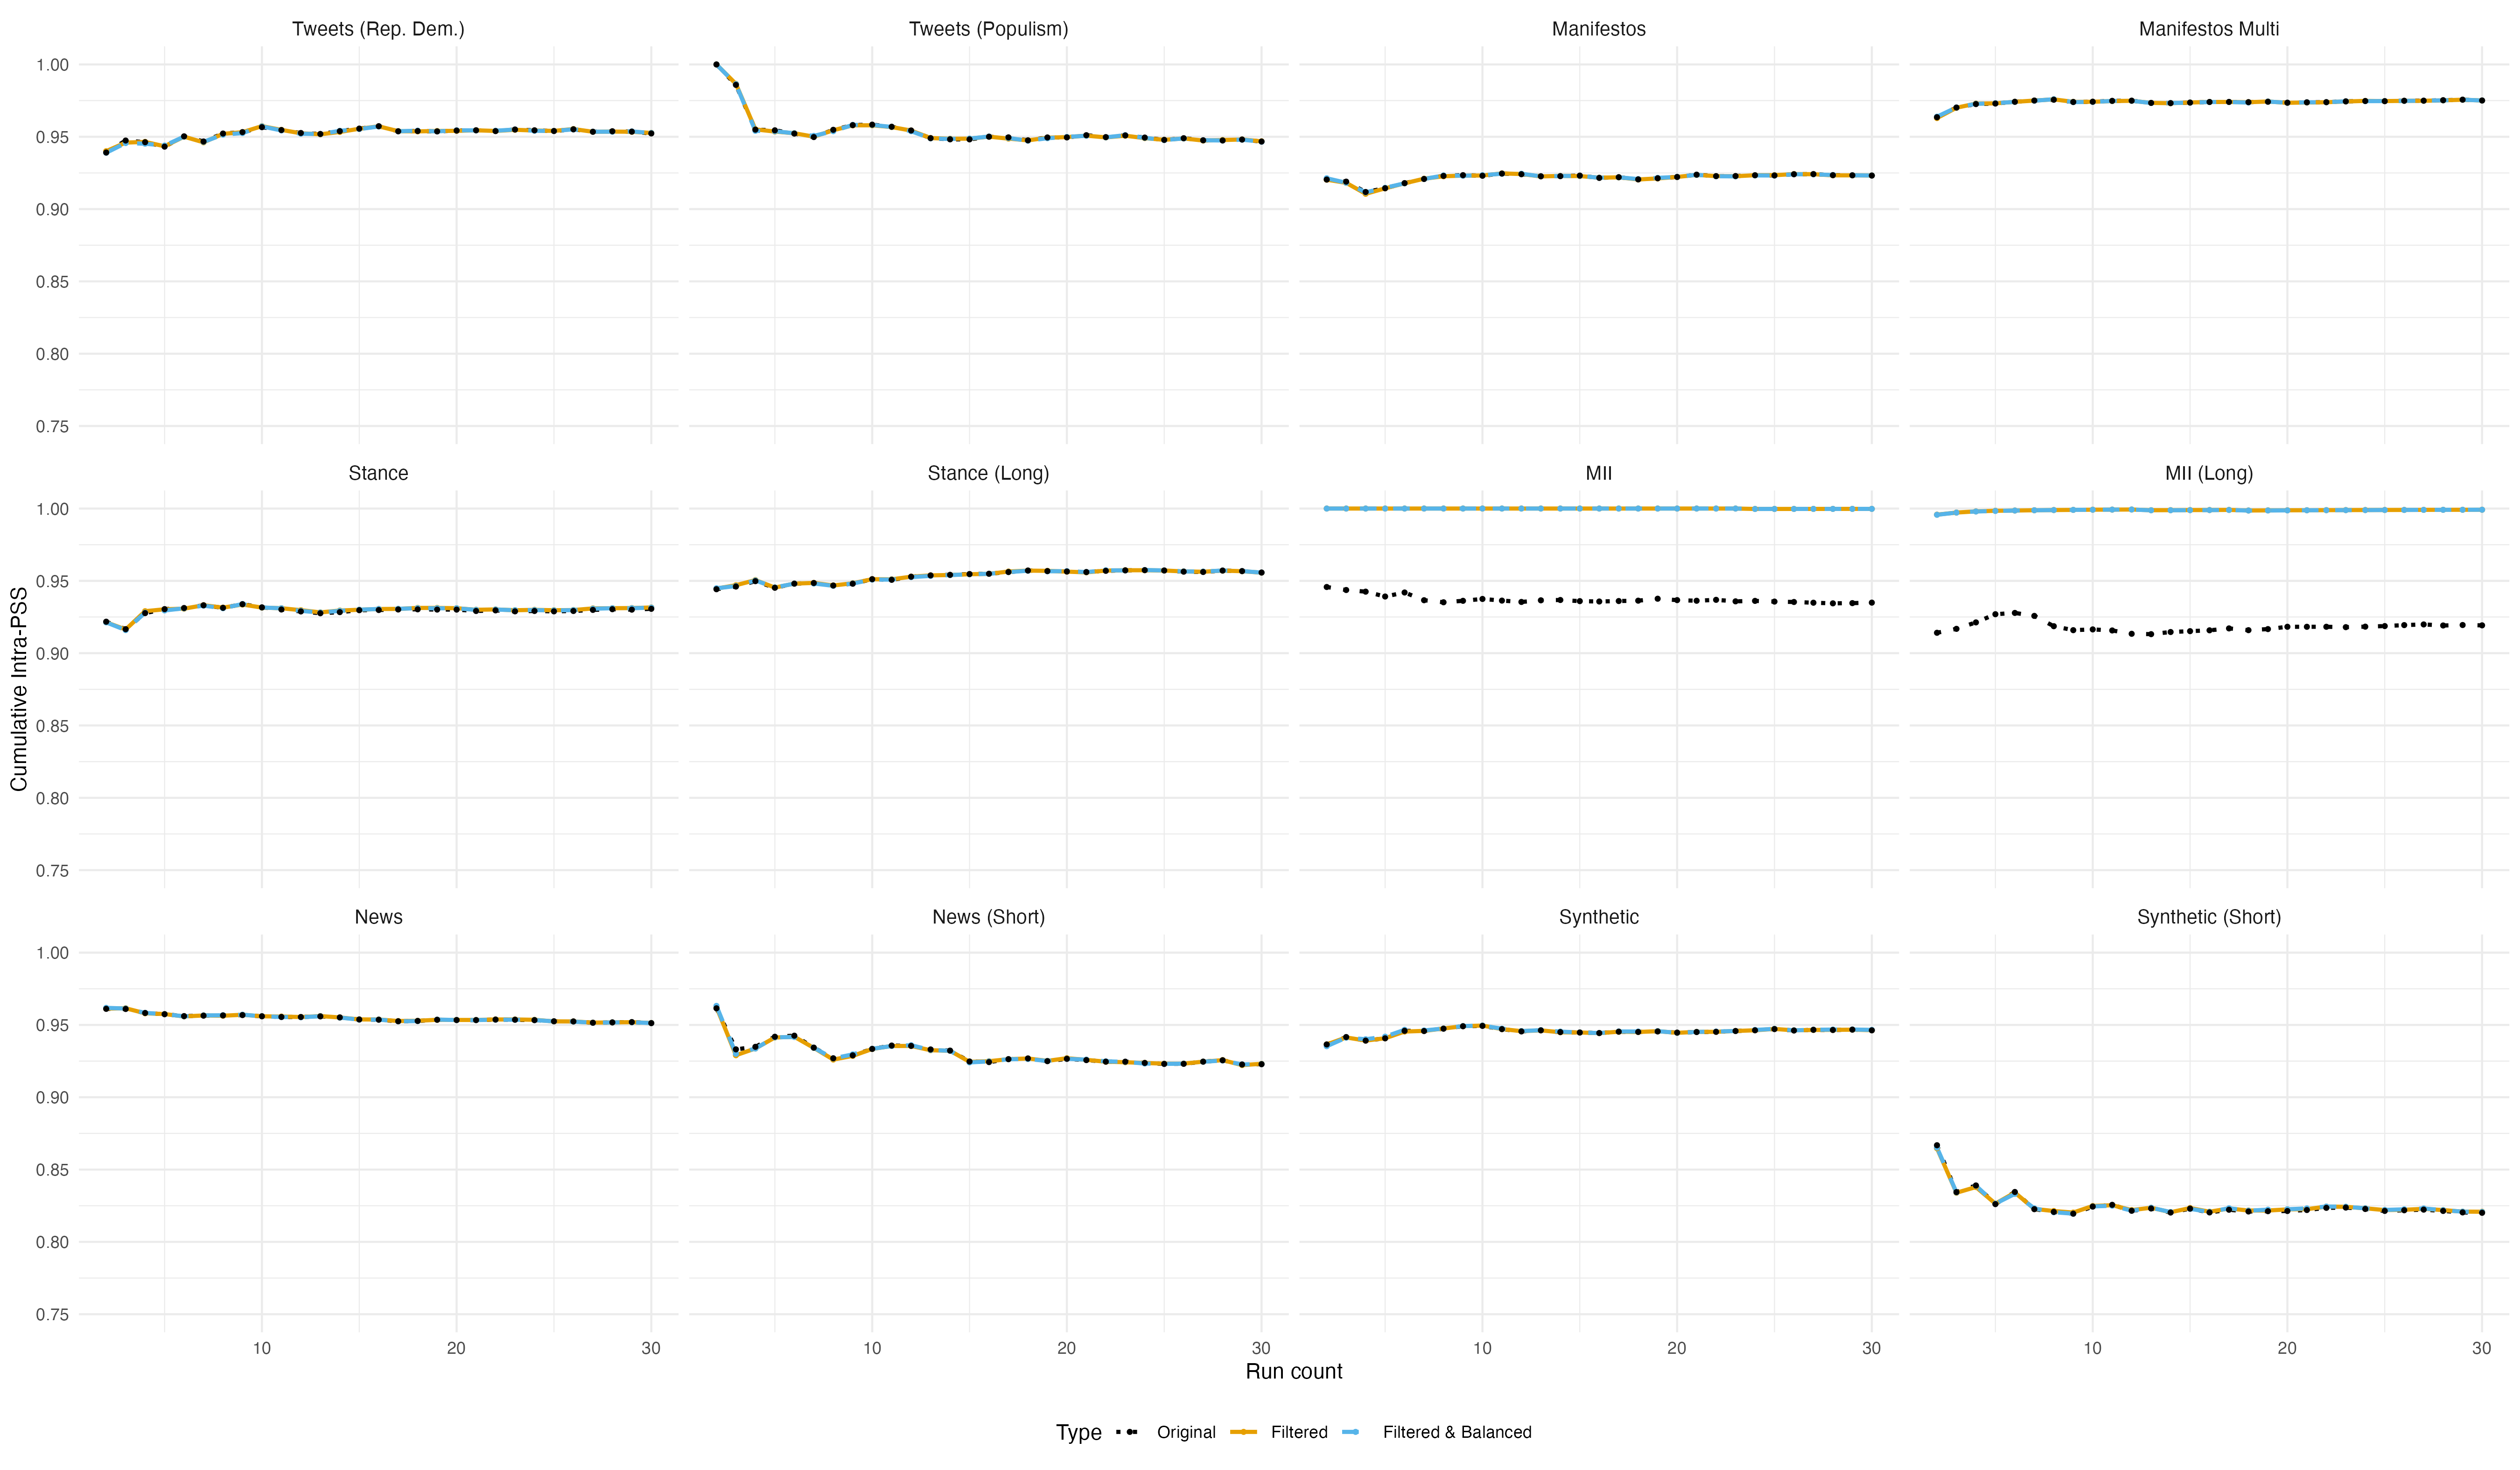
\includegraphics[width=1\textwidth]{plots/combined_within_postpro_cumulative.png}
    \caption{Filtered diagnostic comparison for cumulative intra-prompt stability.}
    \label{fig:combined_within_postpro_cumulative_appendix}
\end{figure}

\begin{figure}[ht]
    \centering
    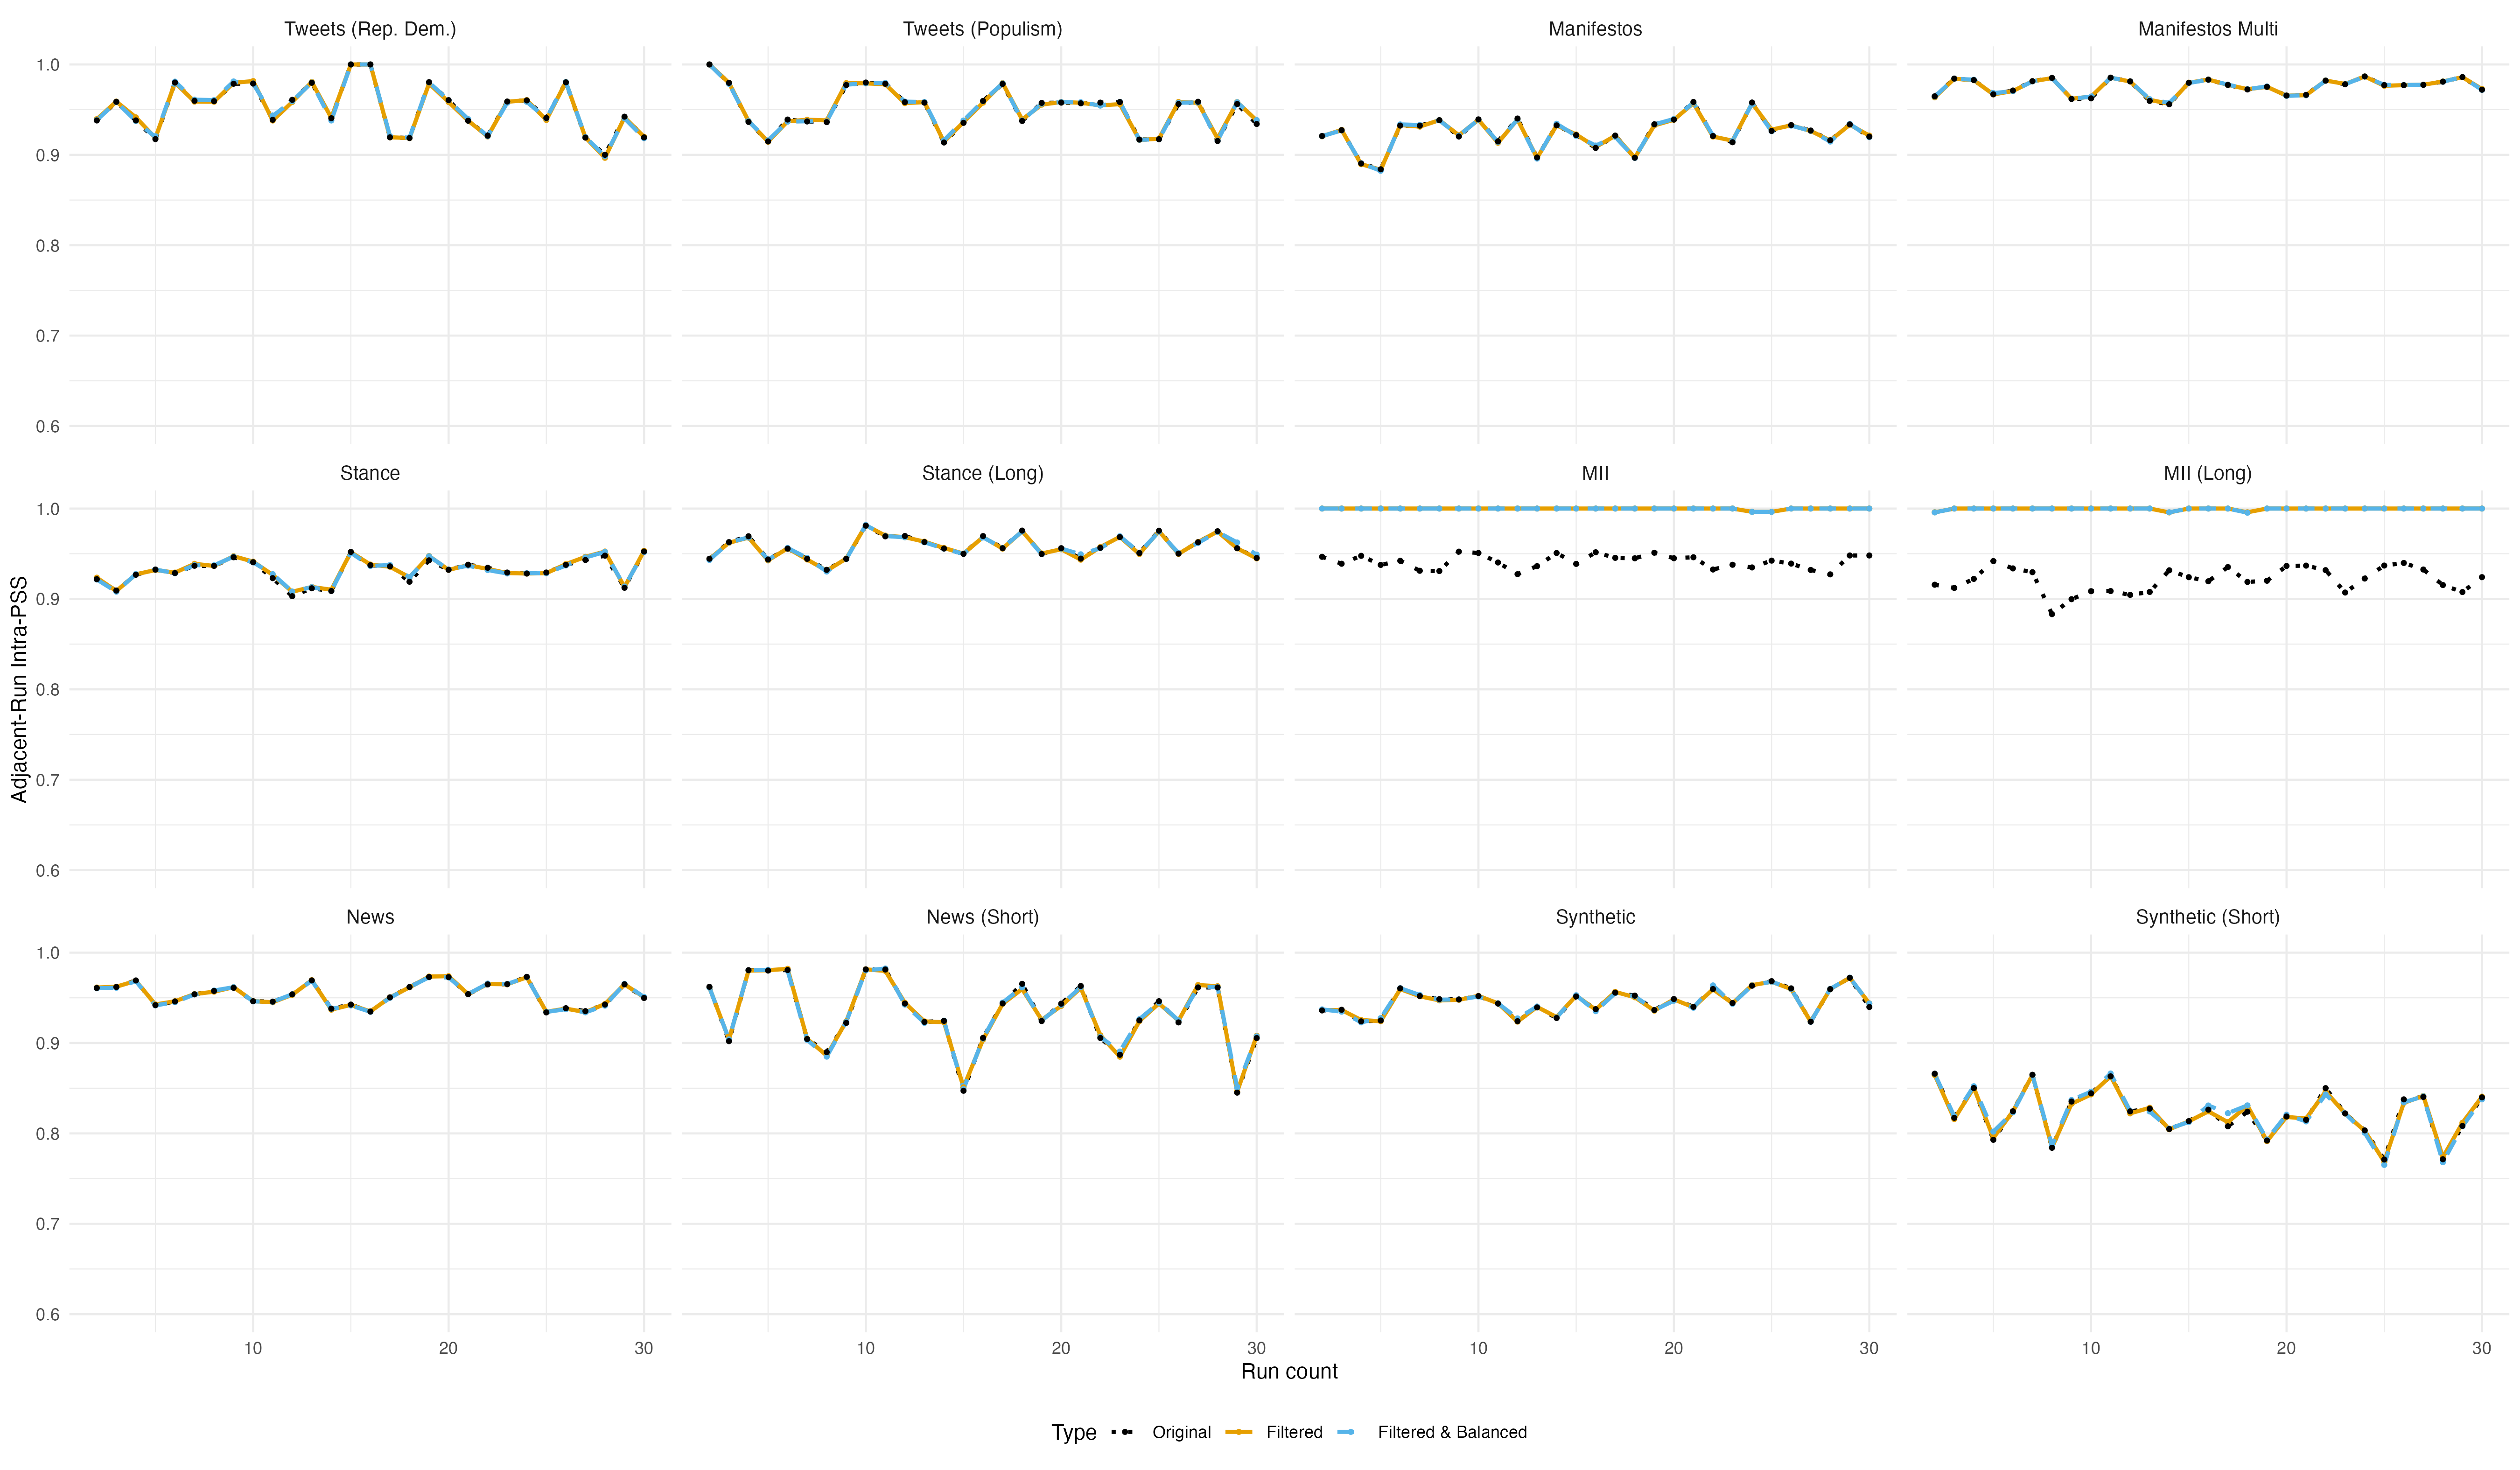
\includegraphics[width=1\textwidth]{plots/combined_within_postpro_adjacent.png}
    \caption{Filtered diagnostic comparison for adjacent-run intra-prompt stability.}
    \label{fig:combined_within_postpro_adjacent_appendix}
\end{figure}

\begin{figure}[ht]
    \centering
    
\includegraphics[width=1\textwidth]{plots/combined_between_postpro.png}
    \caption{Filtered diagnostic comparison for inter-prompt stability.}
    \label{fig:combined_between_postpro_appendix}
\end{figure}

\subsection{Are other LMs more stable?}

In our main analyses, we find that---for some datasets---the inter-PSS decreases even at low temperatures. One might expect that the latest commercial LMs would perform better than the LM we use (\texttt{gpt-3.5-turbo}), which has since been surpassed by newer models. To test this conjecture, we take the four worst (post-filtering) performing dataset and outcome pairings (News (Short); News; Stance (Long); and Synthetic (Short) and re-estimate the inter-PSS using \texttt{gpt-4o-mini}. We see in Figure \ref{fig:combined_between_updated} that while this model produces annotations that are indeed more stable, the Synthetic (Short) data is about as stable as in the main analyses. 

\begin{figure}[ht]
    \centering
    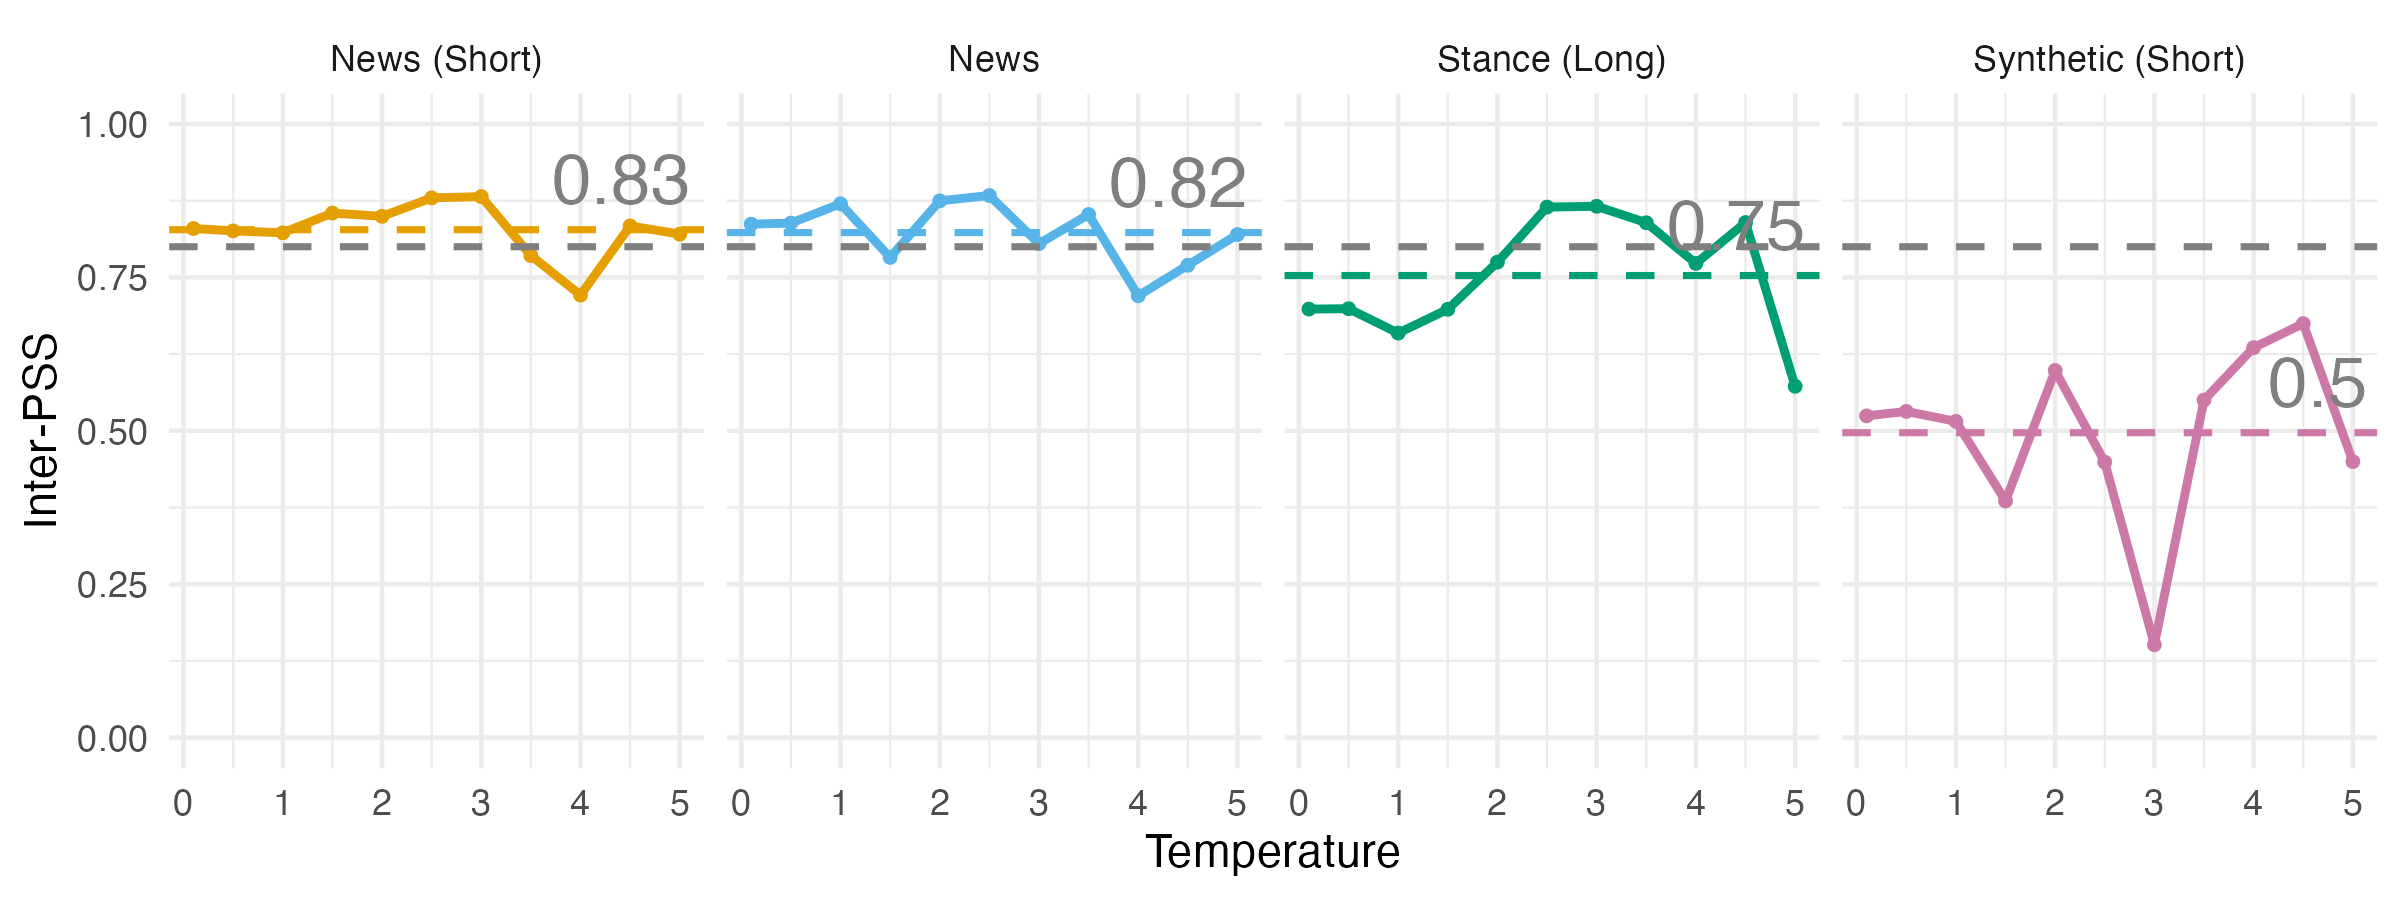
\includegraphics[width=1\textwidth]{plots/combined_between_updated.png}
    \caption{Combined inter-prompt stability scores for lowest inter-PSS outcomes in post-filtering analyses.}
    \label{fig:combined_between_updated}
\end{figure}

It should be noted that while PSS is not a measure of accuracy, it provides a crucial dimension of model evaluation: the stability and reproducibility of a model's outputs. When choosing between language models, researchers can compare their intra- and inter-PSS profiles to assess which model generates more stable classification for a given task. A model that produces highly unstable outputs cannot be trusted to yield accurate classifications, regardless of its average performance on benchmark datasets. We therefore recommend that researchers treat PSS as one dimension of model selection, alongside accuracy, cost, speed, and domain suitability. The main text provides a limited cross-model comparison between \texttt{gpt-4o} and \texttt{deepseek-r1:8b}; the appendix analysis here is intended as a supplementary robustness check using a newer commercial model.

\section{Prompt variants}

The prompt variants we used for the main analyses can be found at the anonymized Github repo: \url{https://anonymous.4open.science/r/promptstability-7AD3}.

\tiny
\clearpage
\section{Original prompts}

\input{inputs/original_prompts}
